\documentclass[10pt]{article}
\usepackage[usenames]{color} %used for font color
\usepackage{amssymb} %maths
\usepackage{amsmath} %maths
\usepackage[utf8]{inputenc} %useful to type directly diacritic characters
\usepackage{tikz}
\usetikzlibrary{arrows,positioning,decorations.pathreplacing}

\definecolor{boiseBlue} {RGB}{29,72,159}
\definecolor{rojoAmor} {RGB}{171,13,4}
\definecolor{moradoAmor} {RGB}{93,8,113}
\definecolor{verdeAmor} {RGB}{98,158,31}
\definecolor{negro} {RGB}{10,10,10}
\definecolor{lgreen} {RGB}{180,210,100}
\definecolor{dblue}  {RGB}{20,66,129}
\definecolor{ddblue} {RGB}{11,36,69}
\definecolor{lred}   {RGB}{220,0,0}
\definecolor{nred}   {RGB}{224,0,0}
\definecolor{norange}{RGB}{230,120,20}
\definecolor{nyellow}{RGB}{255,221,0}
\definecolor{ngreen} {RGB}{98,158,31}
\definecolor{dgreen} {RGB}{78,138,21}
\definecolor{nblue}  {RGB}{28,130,185}
\definecolor{jblue}  {RGB}{20,50,100}\begin{document}
\[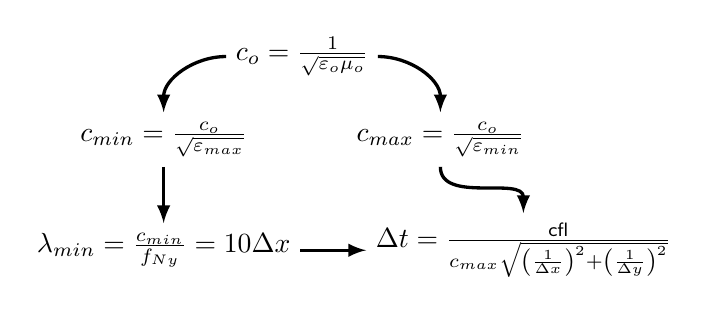
\begin{tikzpicture}[>=latex]
%
\node[minimum size=0.5cm] at (0,0)  (co) {$c_o = \frac{1}{\sqrt{\varepsilon_o\mu_o}}$};
\node[minimum size=0.5cm] at (-5em,-3em)  (cmin) {$c_{min} = \frac{c_o}{\sqrt{\varepsilon_{max}}}$};
\node[minimum size=0.5cm] at (5em,-3em)  (cmax) {$c_{max} = \frac{c_o}{\sqrt{\varepsilon_{min}}}$};
\node[minimum size=0.5cm] at (-5em,-7em)  (lmin) {$\lambda_{min} = \frac{c_{min}}{f_{Ny}} = 10\Delta x$};
\node[minimum size=0.5cm] at (8em,-7em)  (dt) {$\Delta t = \frac{{\sf cfl}}{c_{max}\sqrt{ \left(\frac{1}{\Delta x}\right)^2 + \left(\frac{1}{\Delta y}\right)^2}}$};
%
\draw[->,very thick,black]
  (co) to[out=180,in=90] (cmin);
\draw[->,very thick,black]
  (co) to[out=0,in=90] (cmax);
\draw[->,very thick,black]
  (cmin) to[out=270,in=90] (lmin);
\draw[->,very thick,black]
  (lmin) to[out=0,in=180] (dt);
\draw[->,very thick,black]
  (cmax) to[out=270,in=90] (dt);
%
\end{tikzpicture}
\]
\end{document}